\chapter{16 Tales 1}

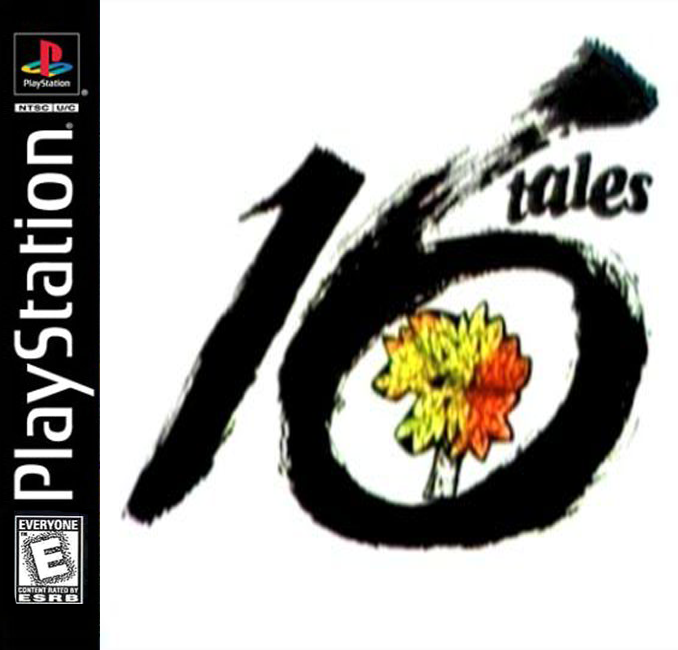
\includegraphics[width=\textwidth/2]{"./Games/16Tales/16TalesGeneralLogo.png"}

The first of the four 16 Tales games published and released by The Lightspan Partnership for the PlayStation 1. Each game consists of four 15-minute video programs various cultures' stories and lore.

16 Tales 1 features a series of four Native American stories, including:
\begin{itemize}
    \item The Angry Moon %\href{https://www.goodreads.com/book/show/24890.The_Angry_Moon?from_search=true & from_srp=true              & qid=GFQW4v18PS   & rank=1}{Link to equivalent book on Goodreads} \\
    \item Coyote and Cottontain \& Coyote and the Beaver People
    \item The Dancing Stars \& The Friendly Wolf
    \item The Fire Bringer \& How Saynday Borought the Buffalo to the Indians
\end{itemize}

Music used throughout:
- Sun Valley by David Snell

\begin{table}[h]
    \centering
    \begin{small}

        \begin{tabular}{|p{1.5cm}|p{8.5cm}|p{7cm}|}
            \hline
            \textbf{Story Title} & \textbf{Short Description} & \textbf{Credits} \\
            \hline
            The Angry Moon
                                 &
            A story based on a Native American legend from the Tlingit people in Alaska.
            Adapted from a legend of the Tlingit Indians of Alaska, this book follows Lupan and Lapowinsa and their adventure to the sky country.
            Lupowinsa laughs at the moon and is taken as prisoner by the Moon as punishment.
            Fearing his friends welfare, Lupan makes a ladder of arrows up to sky country.
            With the help of old grandmother, Lupan is given four gifts to help defeat the Moon and save his friend.
                                 &
            Told by: Ginny Taylor,
            Producer: K. Hamamura Nelson,
            Executive Producer and Director: Edmond R Chavanette,
            Story Editor: Toni Lonehawk Eagleshield,
            Illustrator: Peggy Ostermann, PhD.,
            Titles and Set: Doug Stiles,
            Lighting: Ron A. Vanicek,
            Technical Director: Bill Bolle,
            Audio: Larraine E. Wilson,
            Video: Roger Knipp,
            Videotape: Clarence Pemberton,
            Camera: John C. Merritt, Martin Miller, Ron A. Vanicek,
            KLCS Los Angeles Unified School District
            \\
            \hline
            Coyote and Cottontail \& Coyote and the Beaver People
                                 &
            Based on Navajo stories.
            Coyote and Cottontail is a story about a wolf who tries to chase a rabbit.
            Coyote and the Beaver People is a story about a wolf who is skinned by a group of beavers.
                                 &
            Told by: Ginny Taylor,
            Producer: K. Hamamura Nelson,
            Executive Producer and Director: Edmond R Chavanette,
            Story Editor: Toni Lonehawk Eagleshield,
            Illustrator: Joe Whitecloud Tafoya,
            Titles and Set: Doug Stiles,
            Lighting: Ron A. Vanicek,
            Technical Director: Bill Bolle,
            Audio: Larraine E. Wilson,
            Video: Roger Knipp,
            Videotape: Clarence Pemberton,
            Camera: John C. Merritt, Martin Miller, Ron A. Vanicek,
            KLCS Los Angeles Unified School District
            \\
            \hline
            The Dancing Stars \& The Friendly Wolf
                                 &
            The Dancing Stars is an Iroquois legend.
            Seven brothers follow a celestial lullaby into the sky, where they encounter the Great Bear and face a choice between home and the stars.
            The Friendly Wolf is a story that comes from the Dakota people.
            Siblings Little Cloud and Bright Eyes befriend the Great Wolf during a storm in the mountains.
            Guided safely home, their encounter fosters a lasting bond between their people and the wolves.
                                 &
            Told by: Dennis Wilkerson,
            Producer: K. Hamamura Nelson,
            Executive Producer and Director: Edmond R Chavanette,
            Story Editor: Toni Lonehawk Eagleshield,
            The Dancing Stars Illustrators: Holylight \& Sam Barcelo,
            The Friendly Wolf Illustrator: Charles E. Brown,
            Titles and Set: Doug Stiles,
            Lighting: Ron A. Vanicek,
            Technical Director: Bill Bolle,
            Audio: Larraine E. Wilson,
            Video: Roger Knipp,
            Videotape: Clarence Pemberton,
            Camera: John C. Merritt, Martin Miller, Ron A. Vanicek,
            KLCS Los Angeles Unified School District
            \\
            \hline
            The Fire Bringer \& How Saynday Borought the Buffalo to the Indians
                                 &
            The story revolves around two Native American legends: "The Firebringer" from the Paiute tribe and "How the Buffalo Came to the Indians" from the Kiowa tribe.
            In "The Firebringer," an Indian boy seeks to help his people who are suffering in the cold winter without fire.
            With the guidance of Coyote, they embark on a dangerous journey to obtain fire from a burning mountain.
            Despite initial skepticism, they succeed in bringing fire back to their tribe, earning the boy the name "Firebringer."
            In "How the Buffalo Came to the Indians," Sand Day, observing the suffering of animals due to hunger, devises a plan to discover the source of White Crow's abundant food.
            Through trickery, Sand Day uncovers a hidden stash of buffalo meat, leading to the release of the buffalo to roam freely and provide sustenance for the Native American tribes.
            Both stories highlight the importance of survival, resourcefulness, and the interconnectedness between humans and nature in Native American folklore.
                                 &
            Told by: Dennis Wilkerson,
            Producer: K. Hamamura Nelson,
            Executive Producer and Director: Edmond R Chavanette,
            Story Editor: Toni Lonehawk Eagleshield,
            The Firebringer Illustrators: Holylight \& Natche Stan Salazar,
            How Saynday Borought the Buffalo to the Indians Illustrator: Lavona Thomas,
            Titles and Set: Doug Stiles,
            Lighting: Ron A. Vanicek,
            Technical Director: Bill Bolle,
            Audio: Larraine E. Wilson,
            Video: Roger Knipp,
            Videotape: Clarence Pemberton,
            Camera: John C. Merritt, Martin Miller, Ron A. Vanicek,
            KLCS Los Angeles Unified School District,
            \\
            \hline
        \end{tabular}
    \end{small}

\end{table}

\clearpage
\newpage

\section{Transcriptions}

\subsection{The Angry Moon}

Today's story is about "The Angry Moon". It is from the Tlingit Indians of Alaska.

The moon plays an important part in the lives of the Tlingits because most of their food comes from the sea. The moon was considered to be a powerful God to be reckoned with. The Tlingits have a very rich culture and a strong imagination.

In today's story, look for the many beautiful examples of Tlingit designs. You will notice the symbol of an eagle perched on the bow of a boat, on the totems, and on the grandmother's house. This design is based on an old Tlingit legend of "Eagle Woman", who turned herself into an eagle in order to save her children.

The design on grandmother's dress is from a spoon, because you see, the Tlingits made beautiful in-sized spoons out of animal horn. And you will see faces which look like ceremonial masks. In many Indian legends, people are transformed into animals and other beings in order to accomplish their goals. The masks worn in ceremonies which depict these tales are called "transformation masks".

Look for the moon crest on the moon's house, and a whale design on the blankets. In fact, be sure to watch very closely. You'll see designs representing the Northwest Coast Indians throughout the entire story.

But apart from the designs, "The Angry Moon" may be similar to other stories, stories that you've heard before. Tell me if it is. It's now time to listen to the tale of "The Angry Moon".

One very bright summer night, when the moon was full, Lupan and La puinsa were walking in the grassy country that surrounded their village. They were good friends. Tonight, the moon was full and especially bright. It almost seemed to be watching them. Lupan laughed and said, "What a funny face the moon has. How ugly it is."

"Be quiet," said Lupan. "It is not good to speak badly about the moon."

Suddenly, the field was covered in darkness, and a strange, shimmering rainbow appeared from out of the shadows and surrounded La puinsa. She was frightened and cried out for Lupan. He stepped toward her, and the rainbow disappeared, and the darkness disappeared, and La puinsa disappeared. Lupan was all alone in the bright moonlight. He called and called, but there was no La puinsa.

He ran to the top of a hill and cried, "The moon has taken her!" He thought. As his tears dried, he looked up at the sky and saw a brilliant star right beside the Moon. A strange idea came into his mind. "I wonder if I can hit the star..." He took out his bow and arrow and, aiming very carefully at the star, shot at the star. The star disappeared. Strangely, his arrow did not come back. Again and again, Lupan shot his arrows towards the empty space where the star had been. The arrows never, never returned.

Lupan had been shooting arrows all night, and with the first rays of the morning sun, the line of arrows turned into a ladder leading up to the sky. Without knowing why, Lupan picked some branches from a nearby bush and put them in his hair, and then he began to climb the ladder up into the sky. He was afraid. Powerful winds made the ladder spin around. A sudden rainstorm poured down on him, and the ladder became wet and slippery. He hung on tightly and did not fall.

He was still climbing the ladder when night came. Lupan wrapped himself about the ladder and fell asleep. The sunrise of another day shone on Lupan. He had never seen the Sun so bright. The heaviness of his head made him reach up to touch it. He put his hand up to find that the branches in his hair had grown into bushes full of big, sweet berries. He was amazed, but he was also very hungry, so he ate the berries and threw away the branches.

All day long he climbed above the clouds. At nightfall, he reached the top of the ladder. He was very tired, so he lay down and fell asleep. He was awakened by a small voice. "Wake up, I am coming for you. Wake up, my grandmother wishes me to bring you to her. She has been watching you climb here from Earth."

Lupan was very surprised. There was a small boy looking at him, and so Lupan followed the boy over the sky road to the grandmother's house. She was glad to see Lupan and welcomed him. They sat around the fire. The grandmother said, "It is I who helped you on your way to this country. I could tell you were brave and had great need to come up to the sky."

"I have come to find La puinsa," said Lupan

"Yes," said the grandmother, "she has been captured by the moon, who lives near here." They could hear La puinsa's voice wailing in the distance. Lupan wanted to go to her, but the old grandmother told him to eat first to regain his strength. She raised her hand three times, and each time food appeared: first a fish appeared, then a toasted ear of corn, she raised her hand a third time and fresh fruit appeared. Lupan ate hungrily and felt refreshed.

"Now, when you go to the house of the Moon, you must take four things." The grandmother gave him a pine cone and a fisheye, then a rose and a small stone. He was to use these to help him rescue La puinsa. Lupan hurried into the land of the Moon. The closer he came to the moon's house, the louder La puinsa's cries became, and he began to run. Now he could see her up on the roof, caught in the smoke hole with the fire licking at her heels.

He quietly ran to the roof so that the moon could not hear him. La puinsa was so happy to see him, she stopped crying. "Don't stop crying," Lupan whispered. "Cry louder. I don't want the moon to know that you are getting away." So she cried louder as Lupan pulled her from the smoke hole. He put the pine cone in the smoke hole, and it made a crying sound just like La puinsa.

Hand in hand, they started to run. Then the pine cone stopped crying, and the moon became very angry. He had been tricked. He thundered out of his house, chasing after La puinsa and Lupan. He rolled much faster than they could run. Lupan turned and threw the fisheye at him, and where it fell, a large lake appeared. The moon was going so fast, he could not stop and rolled into the lake. He was wet and cold as he rolled out of the lake. He had to roll around the lake, but he was fast. He quickly caught up to Lupan and La puinsa. Lupan threw the rose at the moon, and he became tangled in roses and thorns.

As he came through them, he was very angry. He rolled even faster. When Lupan saw the moon behind them, he threw the stone at the moon, and a huge mountain appeared. It was too high for the moon to climb. It just rolled up and down again.

Tired and breathless, Lupan and La puinsa finally reached the grandmother's house. They were welcomed by the grandmother and the child, and they rested. Then the grandmother said, "Your ladder is waiting for you. You may return to your home on Earth if you wish." They said goodbye and started to climb down the ladder, down through the thick, puffy clouds.

As they reached the Earth, the sun was setting. The rays of the Sun touched the ladder, and it disappeared, leaving a pile of arrows on the ground. The children picked them up and put them in their quivers, then they joyfully ran home. The people of the village were very happy to see them, and for the rest of their lives, people came from far and near to hear their story about "The Angry Moon". The story is still told in the village today.

Did this story remind you of other stories you've heard before? I'll bet it did. "The Angry Moon" may have reminded you of "Hansel and Gretel". You see, stories from all over the world can be very similar. In the American Indian tribes, the storytellers were considered very important people because all of the stories have such deep meanings. The Indians respected the storytellers and loved them.

Look forward to Tlingit and other stories of the Northwest Coast Indians. You can find them in your school or public library. Share a story with a friend so our tales will never end.

\subsection{Coyote and Cottontail \& Coyote and the Beaver People}

The Navajo Indians are from the southwestern part of the United States, mainly Arizona and New Mexico. They are excellent farmers and artists, well known for their turquoise and silver jewelry and for their weaving. The beauty of their rugs is known all over the world.

Our first story is a Navajo legend about our good friend "Coyote". "Trotting Coyote", as he is called by the Navajo, is used as an example of how not to be. He tries to cheat and trick and always loses in the end. In our second legend, we will see what happens to Coyote when he meets the beaver people. Listen now to the tales of "Coyote and Cottontail" and "Coyote and the Beaver People".

One day, Trotting Coyote was sitting on a riverbank. He was very hungry and sad because he had not eaten all day. He had not caught a single cottontail or even a tiny mouse. All of a sudden, a cottontail jumped from the bushes where he was hiding and kicked up a great cloud of sand right in Coyote's face. Coyote ran after the cottontail, thinking, "Hmm, what a delicious dinner that cottontail will make."

Coyote was much faster than Cottontail and easily caught him. Just as he was about to take a bite out of the rabbit, the rabbit said, "Stop, don't eat me."

Coyote was so surprised he almost dropped the rabbit. "Rabbits don't talk," he thought. "What a strange rabbit." First, he jumped from a bush where he could have hidden, and now he's talking. Coyote decided to hear what the rabbit had to say.

"You'll be sorry if you eat me," said the Cottontail. "I have no meat on my bones. Why be in such a hurry? I can't escape from you. You are much too big and strong. I'd like to talk to you for a while, but you are squeezing me too hard."

"What do you want to talk about?" said Coyote, as he stopped squeezing a little. The Cottontail thought fast. He was trying to think of a way to escape.

"Uh, let's talk about people. I know all about people."

"I know much more about people than you do," said Coyote, and he squeezed a little harder.

The Cottontail said, "You think you know so much about people? Why, I'll bet you think they carry their weapons on their backs."

"That's right, on their backs," said Coyote.

"And I'll bet you always stay as far away from people as you can. You never really see their weapons. That's why you are wrong. I have seen them carry their weapons in their hands." Cottontail was trying to keep Coyote's mind off his empty stomach. Coyote was squeezing him tightly again.

Cottontail said, "Stop squeezing me so hard, cousin. You have me, and I can't escape. Let me talk for a little while longer, then you may eat me."

Coyote said, "I'll let you talk more about people and their weapons, but make your story very short." Coyote was very annoyed.

Cottontail was trying not to show how scared he was. He sure didn't want to be eaten. "Well, cousin," said Cottontail, "um, what they do is carry a bow and arrow. They hold a bow up, put the arrow at the bowstring, and pull it as hard as they can, and then the arrow flies to its mark."

Coyote said, "No, that's not the way it is. They carry the bow and arrows on their backs and they shoot from over their shoulders."

Cottontail thought to himself, "Here's my chance to escape." "Stop holding me so tightly, and I will show you how it's done," said Cottontail. Coyote loosened his grip as Cottontail raised his arms. Then Cottontail jumped to the ground and ran away as fast as he could.

Coyote chased the rabbit in and out of the bushes, but he never quite caught him. Then Cottontail kicked a thorny yucca plant right into Coyote's mouth. While Coyote was trying to spit out the yucca needles, Cottontail ran into a small cave in the rocks. Coyote couldn't go in after Cottontail because he was too big, so he pretended he wanted to talk.

"Cottontail," said Coyote, "I um, no, you don't really want to talk, you want to eat me."

"If you don't come out, I'm going to smoke you out with cedar bark or sagebrush," said Coyote.

"Oh good, cedar bark and sagebrush are my favorite foods," said Cottontail.

"Hmm, then I'll get some pinion pitch, that will fix you," said Coyote.

Cottontail pretended to be afraid. Coyote piled some rocks in front of the small opening, then he went to get the pitch. Soon he returned and made a fire and placed the pitch on it.

Cottontail pretended to cry, "Oh, please don't blow the smoke on me. I won't be able to breathe."

Coyote blew the smoke into the crack where the rocks were. Cottontail pretended to cough, but he wasn't getting any of the smoke because Coyote was blowing it into the rocks.

Cottontail said, "Blow harder so it will be all over."

Coyote got as close to the fire as he could and blew and blew. He could just taste that rabbit. Suddenly, Cottontail pushed the hot rocks. They fell into the fire and Coyote's face. Cottontail jumped past Coyote and escaped. It took Coyote a long time to get the smoke and dirt from his face. He didn't clean his face very well. He was too busy thinking of the dinner he had lost. That's why to this very day, the coyote has black streaks on his face.

On another day, Trotting Coyote was sitting near a little pool, picking flowers and watching some beaver people playing the hoop and pole game. He had not played the hoop and pole game for a long time. Coyote sat down near the beavers and asked them, "Uh, what is the prize for getting the pole through the hoop?"

A beaver answered, "The loser is skinned by the winner."

Coyote was surprised. "Oh, I wouldn't want to be skinned."

The beavers thought they were rid of Coyote, so they continued playing. One of them threw the pole through the hoop as it was moving. He was the winner, so he began skinning the loser. The loser jumped into the water as soon as he was skinned, swam around a little up and down, in and out, and suddenly grew a new skin.

Coyote thought to himself, "Hmm, since I have magical powers, I'll bet I could grow a new skin too. I think I'll play with them."

An old beaver warned Coyote not to play. He told him to go and play his own games. Coyote begged the beavers to let him play. After much begging, the beavers said yes. They gave Coyote a pole and began rolling the hoop. Coyote threw the pole and won. He didn't know the beaver people had let him win on purpose.

"I knew I would win," boasted Coyote. "I don't want to skin anyone, but I will play another game."

The old beaver said, "If you lose, you will be skinned, and that can hurt if you're not a beaver, so I think you should stop now."

Coyote said, "Now, just grow a new skin like you beavers do."

They let him play again, and he lost. Coyote suddenly decided that he did not want to be skinned, but it was too late. Coyote yelled and howled and sure made a lot of noise.

His skin was finally peeled from him. Coyote ran for the water as soon as they had him peeled. He swam around a little up and down in and out, but nothing happened. He got out of the water and jumped in again, swam around a little up and down and in and out, but still nothing. He didn't get a new skin.

Seeing how upset he was, the beaver people decided to help him. The old beaver said, "Badger has extra skins in his badger hole. Maybe he will give you one. It won't hurt to ask."

Coyote agreed. He didn't care what kind of skin he got as long as he got something to cover his skinless body. So they all went over to the badger hole, and Coyote went inside. When he finally came out, he was wearing a badger skin. To this day, the badger and the coyote have the same kind of skin.

Storytellers were very important people in all Indian tribes. They were respected for their wisdom, and they were loved. Their stories had such deep meanings. In fact, all of the customs and beliefs of the Indian had a story or legend behind them. There were lessons for everyday living woven into interesting stories. The primary concern of all tribes was to live in harmony with the Great Spirit and all that he created.

Go read and enjoy "Legends of the American Indian". You can find them in your school or public library. Share a story with a friend so our tales will never end.


\subsection{The Dancing Stars \& The Friendly Wolf}

To the American Indian, all animals and nature—the sky and the Earth, all the creatures that walk, crawl, or fly—were important to everyday life. They were thought of and talked of as though they were real people.

Our first story, "The Dancing Stars," is an Iroquois legend. To the great Iroquois nation in the northeastern part of the United States, the Great Bear sang, and the moon smiled and talked. Everything was a creation of the great spirit.

Our second story, "The Friendly Wolf," comes from the Dakotas, where we find the Plains Indians. Their beliefs were the same as their Iroquois cousins. They respected all animals, and they learned to live with them. The Plains Indians are made up of tribes that we've all heard of: the Sioux, or Lakota; Blackfoot; Cheyenne; Pawnee; the Cree; the Nez Perce; Kiowa; Comanche; Crow; the Ojibwe; the Shoshone; the Arapaho; and the Ute, and a few others. They were hunters, depending mostly on the buffalo for their food, clothing, and the covering for their teepees. They also hunted elk, and antelope, and deer. They ate the wild turnip and wild rice. I suppose they're called wild because they were not planted and cultivated by man. They were planted in the ground by the great spirit for our use.

Now, imagine yourself sitting around a flickering indoor fire in the lodgings of your tribe. It is night, which is the best time for storytelling. The old storyteller is about to begin his stories, and it is cold outside. The soft winter snow is lightly falling. In the distance, you can hear the drumming and the singing. You and the other Indians are waiting for the storyteller to begin.

Now listen to the tales of "The Dancing Stars" and "The Friendly Wolf."

Once long ago, when the sky and the stars and the moon and Mother Earth were just beginning, seven brothers were playing in the forest. They loved to run and dance in the forest, always together, never separated. One evening, just as the sun was going down, the brothers heard someone singing. It was a beautiful, beautiful song coming from some far away place. They danced away, following the sound of the music.

Suddenly, it was night. The little boys looked down and saw the trees in their forest, their people's long houses, all the things they knew about, glowing in the moonlight far below them. They were in the sky, still dancing to the strange and beautiful music. They went up and up and up, and the mysterious song grew louder and even more beautiful. They could hear the words clearly now: "Hunter pursued me and I came to the sky, and now I am lost. But I will watch over you in your warm little cave here in the sky. So sleep, little ones, sleep."

Then, they saw a great black bear. Her belt and necklace were made of shiny white clam shells, and her beautiful tail was made of stars. In fact, stars were twinkling at her toes and her nose. It was the Great Bear who was singing the lullaby. They danced long into the night. At last, they stopped, for they wanted to go home. They asked the moon to show them the way, but the moon smiled gently and said, "You will live here in the sky with the stars and I, for we enjoy your dancing."

Suddenly, the boys no longer felt tired, and they no longer wished to go home. They started to dance again, and the Great Bear sang more sweetly than before. Then, a bright shining star grew around each boy.

The smallest brother heard a voice calling his name. It was the voice of his mother. The little boy ran toward the voice as fast as his feet would go, and the star around him left a bright, shiny trail.

"Don't go, don't go," cried the moon and the stars and his brothers, but the little boy would not listen. He fell past the clouds and the trees, reaching for the earth and the sound of his mother's voice. He saw his mother and reached out to take her hand. Then, he landed. His mother cried when she saw that instead of her son, there was a hole in the ground made by a falling star. She looked up at the sky and called to her other sons, "Stay there, do not come down." She did not want them to become falling stars.

The brothers waved to their mother, for they understood, and they danced on. The mother cried, and her tears fell into the hole where the star had fallen. A little sprout began to grow. It grew faster and faster, taller and taller, up into the sky.

The little brother was now a tree, reaching high into the sky to be with his brothers again. Finally, it reached the Great Bear and the dancing brothers. They were very happy to have their littlest brother back with them. To this day, when you walk through a forest, you will see the pine tree. It is the tallest tree in the forest. And at night, you can see the brothers still dancing to the lullaby of the Great Bear as she sings to her little cubs.

It happened during berry-picking time. This was in the long ago when people and animals lived together and talked to each other. It was the time when the berries were ripe and the camps were set up near the berry bushes, which grew in the valley. The berries were eaten right off the bush.

Little Cloud and his little sister, Bright Eyes, ate all the berries their little stomachs could hold. Little Cloud became tired of berry picking and decided to climb the hills near the valley. He took Bright Eyes with him. They climbed higher and higher to where the grizzly bears and bighorn sheep live. Little Cloud wanted to see the place where the eagles lived, way up on top.

It began to get dark. Little Cloud was afraid. He knew there were mountain lions and wolves in the hills, and the Great Wolf of the mountains. They looked around for a place to stay. It became darker and colder, and Bright Eyes began to cry.

Then, as the owls hooted around them, they saw a small cave. So, they crawled in and went to sleep. Suddenly, Little Cloud was awakened by the loud thunder and cold wind of a fierce storm. In the opening of the cave, he saw the Great Wolf of the mountains. He closed his eyes tightly and prayed that the wolf would not harm them.

As the storm passed, it became quiet. Little Cloud opened his eyes. No wolf. Bright Eyes was still asleep. Maybe he had been dreaming. When the morning came, Little Cloud woke Bright Eyes, and they left the cave quickly. Little Cloud did not tell Bright Eyes of his night visitor, but he knew it wasn't a dream. The tracks in the sand told him so.

As the day went on, they became tired and rested near a stream. The water tasted good. Suddenly, they saw the Great Wolf. Remembering that the wolf did not harm them, Little Cloud said, "Please, Great Wolf of the mountain, we are lost. Help us to return home."

The wolf looked kindly at the children. The Great Wolf reminded Little Cloud of the dogs at camp, with his tongue hanging out and his face smiling. Then, the Great Wolf said, "It was my cave you slept in last night. Have no fear. I will take you home. Stay close to me."

The wolf started off and waited whenever the children fell behind. He would run a little and stop, and run a little and stop. He let Bright Eyes ride on his back when she grew too tired to walk. Then, he led them to berry bushes to eat sweet berries so they wouldn't be hungry. Finally, they reached the top of the hill that they had first climbed. From the hill, they could see their families and friends. They were very, very happy. They wanted the wolf to stay with them, but the Great Wolf refused. He could not go closer to the camp because there were dogs there.

"Anyway, I would not be happy living in a camp. I am a wanderer. I go with my wolf friends to many places. Do not be sad. I will always remember you, and you will hear my call in the early night and think of me."

As the children came down to the camp, the men raced on their horses to meet them. They picked them up and joyfully rode into camp. There was much excitement and happiness at their return. When the people heard Little Cloud's story of how the wolf had saved them, they went to the top of the hill and thanked him. They brought him beautiful gifts and food. The chiefs sat in a circle and smoked the pipe of peace.

It was the sign of friendship forever between the Indians and the wolves. That friendship still lasts.

Wherever the Indians traveled, hunted, laughed, or prayed, it was a tribal affair. They were great believers in togetherness, and that togetherness always included the animals. The storytellers were very important people in all tribes. They were respected for their wisdom, and they were greatly loved. Their stories had deep meanings, for all of the customs and beliefs of the Indians had a story or a legend behind them. Many of these stories are in your school and public library. Go read, enjoy the stories of the American Indian, and share a story with a friend so our tales will never end.

\subsection{The Fire Bringer \& How Saynday Borought the Buffalo to the Indians}

Just as you have favorite fairy tales and stories, the Paiute Indians have long ago loved to hear the old Legends told over and over again.

The Peyote Indians lived mainly in Utah. According to the Paiutes, it was Coyote who taught mankind how to survive on the earth.

Our first story, "The Firebringer," will see how Coyote taught the Indians about fire. The second story is a Kiowa Legend called "How Saynday Borought the Buffalo to the Indians." The Kiowa Indians are Plains Indians. They have lived on the Southern Plains around Oklahoma and Kansas for as long as time itself. They hunted the buffalo. Saynday, who brought many things to the Kiowa, was responsible. Now, listen to the tales of the Firebringer and how Saynday brought the Buffalo to the Indians.

Long ago, in the time of the beginning when animals and humans talked to each other and lived together, there was an Indian boy called the Firebringer. He was of the Paiute Tribe with shiny dark skin and long black hair. He loved to run with a coyote, who was the friend and counselor of his people. They would hunt together in the summer; the boy caught fish with his hands while the women dug delicious roots. In the summer, times were good. Now the winter was not so good. The people were cold and unhappy; this was before the tribes knew about fire.

The boy spoke to the coyote, asking his advice. "How can we help my people? They cannot keep warm in this cold. What can we do?"

The coyote thought, and then he said, "You and I will go to the burning mountain and bring back fire. It will be dangerous, but it is the only way. Gather a hundred strong men and women who are your best runners."

The boy went to gather the runners, but they paid no attention to him; they didn't know what fire was. But the boy continued to talk about the fire, and as the people got colder and colder, one by one, they joined him. Soon, he had his hundred runners.

The coyote explained exactly what was to be done. First in front would be the coyote and the boy; then the fastest runners would follow them, and the slowest would be last.

They went toward the west over the high snow-covered mountains, then through dark windy forests. The runners grew afraid. Coyote said to them, "We will rest here. In the morning, one of you will stay here until the fire comes. You will know the fire because it is red like a rose, but it is not a rose. When you see the fire, you will know it."

In the morning, they headed west, leaving one man to wait for the fire. The people wondered if the fire was an animal or an enemy of some kind.

Coyote explained, "Fire can be an enemy or friend; it can hurt, but it can also help and serve us. If it is covered with rocks and sticks, it can be used to warm the people." The last runner was left to wait for the fire; coyote and the boy continued on to the burning mountain. It was very high with smoke and fire pouring out of its top. At night, the fire spirits danced on the mountaintop. Coyote made himself look thin and weak and unimportant and went up the mountain. The fire spirit saw him but ignored him because he looked harmless.

As the fire spirits began to dance, coyote stole a burning stick and ran down the mountain. The fire spirit saw him running with a fire and began to chase him. Coyote was tired and breathing hard when the boy took the burning stick from his friend and ran with the fire spirits fast behind him.

The boy ran as fast as he could until he came to the runner they had left behind. This runner took the burning stick and ran on. The stick was passed from runner to runner; the fire spirits chased each runner until they were stopped by the snowy mountains. The swift runners continued through the day and night until they came to the land of the Paiute. They surrounded the fire with rocks and put sticks on it and were warmed by it, just as coyote had told them.

From that time on, the boy was called Firebringer. The name Firebringer was passed on to the coyote because he had earned the name.

To this very day, coyote's fur is thin and yellow, as if burned along his sides, perhaps because of the fire stick he carried in his mouth whose flames licked at his sights as he ran down the burning mountain.

Saynday was coming along, and he saw all the animals singing and dancing, and he asked them what they were doing. Owl and Dragonfly told him it was a Sundance to show the Sun how much they loved it. Coyote said, "We are having a fine time, but we are hungry; we have no food."

Fox said, "We are all getting weak because we have no food."

Saynday felt very sorry for the animals as they watched the dancing. He thought of the white crow. "Why is the crow so fat, and his feathers so smooth? He must have plenty of food. Where does he get his food?" Nobody knew.

Now, White Crow always carried a bow and some arrows in a special case, and he never put it down. Saynday decided the answer to White Crow's food must be in the case. Saynday wondered how he could get the case; then he thought of a plan.

He told Fox and Coyote, and Owl and Dragonfly, to watch White Crow when he left the dancing grounds to find out where he lived. They agreed.

Saynday and his friends started to flatter White Crow. "Why aren't you singing? You have such a beautiful voice." White Crow was very pleased to help the singers. Saiyan Day offered to hold the bow and arrow case for White Crow. As White Crow began singing and drumming, all the animals crowded around him, so he couldn't see Saynday. Saynday took the bow and arrows out of the case and laid them down. He reached way into the case and pulled out a piece of meat. Buffalo meat.

He thought to himself, "I have never tasted anything so delicious. This would be good for the Indians." The singing finished, and Saynday gave White Crow his case. As White Crow flew away, Fox and Coyote, and Owl and Dragonfly, all watched; he flew way up and over the nearby hill. Saynday told his friends he would stay behind and think of some way to find out where the buffalo meat was hidden.

He hid near a bush and changed himself into a little puppy. He wanted White Crow's little daughter to find him. Then the little daughter came walking along and saw the puppy. The puppy began licking her ankles, and she picked him up; she wanted to keep him.

But when she took him home, White Crow didn't like him. "I never saw a puppy with a mustache before." Saiyan Day had forgotten to change his mustache. White Crow's little daughter started to cry. So, he agreed she could keep the puppy if she did not take him near the meat.

Saynday ate well that night: Buffalo scraps. The next day, White Crow and his wife had to leave. He said to his daughter, "Remember, don't take the puppy near the meat; that is our secret." Then he and his wife left. Soon, the little White Crow got tired of playing with the puppy. "I'm going to show you our secret place where we keep our meat," Saynday pretended he wasn't interested. The little girl picked him up and took him over to a big deep hole that had been covered with a rock.

Down in the hole were all the Buffaloes in the world, father Buffaloes, mother Buffaloes, and baby Buffaloes. "Indian people should have this food to share; they will never be hungry again." He started barking and jumped down among the Buffaloes. The Buffaloes rushed out of the hole into the sunshine; they sounded like thunder as they ran. White Crow heard the thunder and flew back home as fast as he could; he knew it was the Buffaloes.

As the last Buffalo came up out of the hole, Saynday came out and turned back into himself. He turned to the buffaloes. "You will live here in this country wherever the grass shall grow, to the east, to the west, to the north, and to the south; you will roam; you will be the food for the people of this country."

The Buffalo listened to Saiyan Day; they wandered and spread out over the plains, for they fed and clothed the people. How the Buffalo came to the Indians.

The Indians came to depend on buffalo meat for a large part of their diet and on its skin for clothing, shelter, and many other uses. In winter, the warm skin was used for robes and blankets; no part of the Buffalo was wasted. Without this magnificent animal, the Kiowa as well as other Plains tribes possibly would have died out. Today, you have heard just two stories of the American Indian; you can find many more in your school or public libraries. Go read and enjoy the stories of the American Indian, and share a story with a friend so our tales will never end.

\clearpage
\newpage

\begin{figure}
    \centering
    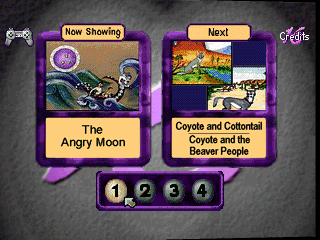
\includegraphics[width=\textwidth/2]{"./Games/16Tales/16Tales1Screenshot.png"}
    \caption{16 Tales 1 Screenshot}
\end{figure}